% Compile with `pdflatex -shell-escape XXXX.tex` in the terminal

\documentclass[crop,margin=4mm,tikz,convert={outext=.svg,command=\unexpanded{pdf2svg \infile\space\outfile}},multi=false]{standalone}

\usepackage[utf8]{inputenc}
\usepackage{todonotes}
\usetikzlibrary{decorations.pathmorphing, decorations.text}
\usepackage{babel}[ngerman]
%\usepackage{fontspec}
%\setmainfont{Arial}
\tikzstyle{every picture}+=[font=\sffamily]


\begin{document}
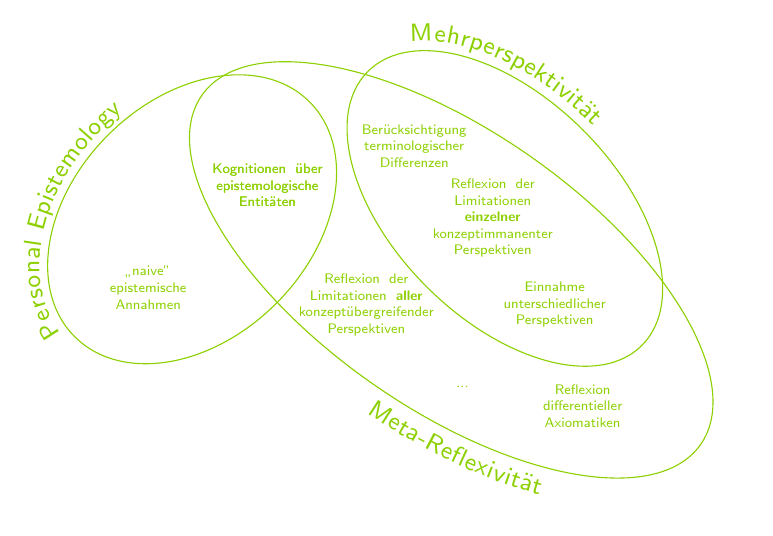
\begin{tikzpicture}
\definecolor{phgreen}{RGB}{140,208,0} 
%%     
\draw[color=phgreen, rotate=+55,
 postaction={decorate,
    decoration={raise=-1em, 
    text along path, pre length=9.3cm,
      text={|\color{phgreen}\sffamily \small|Meta-Reflexivit|\color{phgreen}\sffamily\smallä|t},
    }}] (-0.35,0.3) arc (0:360:50pt and 110pt);  
  
%\setsansfont[Ligatures=TeX]{Arial}
%%     
\draw[color=phgreen, rotate=-135, 
 postaction={decorate,
    decoration={raise=.35em, 
    text along path, pre length=3.7cm,
      text={| \color{phgreen}\sffamily \small|Mehrperspektivit|\color{phgreen}\sffamily\smallä|t},
    },
  }] (2.5,0) arc (360:0:40pt and 70pt);
  


  

%%     
\draw[color=phgreen, rotate=-45, 
 postaction={decorate,
    decoration={raise=0.3em, 
    text along path, pre length=3cm,
      text={|\color{phgreen}\sffamily \small|Personal Epistemology},
    },
  }] (-1.2,-4) arc (360:0:43pt and 60pt);
  


%% Rechteck
 % \draw (-10,-5) --  (3.7,-5) -- (3.7,3) -- node[above] {\Large Topologie} (-10,3) --  (-10,-5);
  
%% Labels
\draw (0,-2) node [text=phgreen, text width=2cm]{  
  \tiny
  \begin{tabular}{c}
     Einnahme\\unterschiedlicher\\Perspektiven
  \end{tabular}};
  
  %% Labels
\draw (-0.9,-0.9) node [text=phgreen, text width=2cm]{  
  \tiny
  \begin{tabular}{c}
     Reflexion der\\Limitationen\\ \textbf{einzelner}\\konzeptimmanenter\\Perspektiven 
  \end{tabular}};
  
    %% Labels
\draw (-2.6,-2.0) node [text=phgreen, text width=2cm]{  
  \tiny
  \begin{tabular}{c}
     Reflexion der\\Limitationen \textbf{aller}\\konzeptübergreifender\\Perspektiven 
  \end{tabular}};
  
  \draw (-0.6,-3.0) node [text=phgreen, text width=2cm]{  
  \tiny
  \begin{tabular}{c}
...
  \end{tabular}};
  
  
  
  %% Labels
\draw (-1.8,-0.0) node [text=phgreen, text width=2cm]{  
  \tiny
  \begin{tabular}{c}
     Berücksichtigung\\terminologischer\\Differenzen\\
  \end{tabular}};
  
%% Labels
\draw (-3.7,-.5) node [text=phgreen, text width=2cm]{  
  \tiny
  \begin{tabular}{c}
     Kognitionen über\\epistemologische\\Entitäten
  \end{tabular}}; 
 
 
 %% Labels
\draw (-3.7,-.5) node [text=phgreen, text width=2cm]{  
  \tiny
  \begin{tabular}{c}
     Kognitionen über\\epistemologische\\Entitäten
  \end{tabular}}; 
 

 %% Labels
\draw (-5,-1.8) node [text=phgreen, text width=2cm]{  
  \tiny
  \begin{tabular}{c}
     \glqq naive"\\epistemische\\Annahmen
  \end{tabular}}; 
 
 \draw (0.5,-3.3) node [text=phgreen, text width=2cm]{  
  \tiny
  \begin{tabular}{c}
     Reflexion \\differentieller\\Axiomatiken
  \end{tabular}}; 
 
 
 
\end{tikzpicture}
\end{document}
